\begin{center}
\begin{tikzpicture}
\draw (2,2) circle (2cm); %big circle
\draw (2,2) ellipse (4cm and 2.5cm); %ellipse
\draw (2,2) circle (0.8cm) node[anchor=south west] {$x_0$};
\filldraw (2,2) circle (2pt); %small circle 1
\draw (2,1.4) circle (0.8cm) node[anchor=south east] at (2.1,1.3) {$a_n$};
\filldraw (2,1.4) circle (2pt); %small circle 2

%drawing lines
\draw (3.936491673, 2.5) -- (7,3) node[anchor=west] {$\mathcal{D}(x_0, r_1)$};
\draw (2.8, 2) -- (7,2) node[anchor=west] {$\mathcal{D}\left(x_0, \dfrac{1}{3}r_1\right)$};
\draw (2.8, 1.4) -- (7,0.75) node[anchor=west] {$\mathcal{D}\left(a_n, \dfrac{1}{3}r_1\right)$};
%adding U node
\node at (4.5,3.5) {$U$};
\end{tikzpicture}\\
\end{center}